\documentclass[aspectratio=169]{beamer}
\usepackage[utf8]{inputenc}
\usepackage[T1]{fontenc}
\usepackage[english]{babel}
\usepackage{booktabs}
\usepackage{graphicx}
\usepackage{pgfgantt}
\usepackage{xcolor}
\usepackage{colortbl}
\usepackage{tikz}
\usetikzlibrary{arrows.meta,positioning,decorations.pathreplacing}

% Theme moderne et épuré
\usetheme{metropolis}
\usepackage{appendixnumberbeamer}

% Couleurs personnalisées
\definecolor{primary}{HTML}{2C3E50}
\definecolor{accent}{HTML}{3498DB}
\setbeamercolor{frametitle}{bg=primary}
\setbeamercolor{progress bar}{fg=accent}

% Couleurs Gantt
\definecolor{thesis}{HTML}{5B9BD5}
\definecolor{done}{HTML}{70AD47}
\definecolor{todo}{HTML}{ED7D31}
\definecolor{review}{HTML}{9673A6}
\definecolor{milestone}{HTML}{C00000}

\title{Thesis Outline}
\subtitle{Public-Data Pretraining for Clinical Information Extraction}
\author{Rian Touchent}
\institute{Sorbonne Université / INRIA Paris (ALMAnaCH)}
\date{January 2025}

\begin{document}

\maketitle

\begin{frame}{Outline}
    \tableofcontents
\end{frame}

\section{Introduction}

\begin{frame}{Introduction}
    \begin{itemize}
        \item Dominant paradigm: pretraining at scale
        \item Healthcare limitation: clinical data is confidential and scarce
        \item Question: can we exploit public data for the clinical domain?
    \end{itemize}
\end{frame}

\begin{frame}{Related Works}
    \begin{enumerate}
        \item Language Models
        \item Corpus Annotation
        \item Clinical Information Extraction
    \end{enumerate}
\end{frame}

\section{Part 1: Building a Biomedical Corpus}

\begin{frame}[plain]
\vfill
\begin{center}
{\Large\textit{Where to find public biomedical text?}}
\end{center}
\vfill
\end{frame}

% ========== CHAPTER 1: Collecting Biomedical Text ==========
\begin{frame}{Ch.1: Collecting Biomedical Text}
    \textbf{Publication:} CamemBERT-bio

    \vspace{0.3cm}
    \textbf{biomed-fr:} First public French biomedical corpus

    \begin{table}
    \centering
    \small
    \begin{tabular}{llr}
    \toprule
    Source & Content & Size \\
    \midrule
    ISTEX & Scientific literature & 276M words \\
    CLEAR & Drug leaflets & 73M words \\
    E3C & Clinical cases \& leaflets & 64M words \\
    \midrule
    \textbf{Total} & & \textbf{413M words} \\
    \bottomrule
    \end{tabular}
    \end{table}

    \vspace{0.2cm}
    $\rightarrow$ Only 2.7 GB (vs 138 GB OSCAR)
\end{frame}

\begin{frame}{Ch.1: NER Results}
    \textbf{Result:} +2.5 F1 avg across 5 benchmarks

    \begin{table}
    \centering
    \small
    \begin{tabular}{llcc}
    \toprule
    Style & Dataset & CamemBERT & CamemBERT-bio \\
    \midrule
    Clinical & CAS1 & 70.50 & \textbf{73.03} \\
    Clinical & CAS2 & 79.02 & \textbf{81.66} \\
    Clinical & E3C & 67.63 & \textbf{69.85} \\
    Leaflets & EMEA & 74.14 & \textbf{76.71} \\
    Scientific & MEDLINE & 65.73 & \textbf{68.47} \\
    \midrule
    \multicolumn{2}{l}{\textbf{Average}} & 71.40 & \textbf{73.94} \\
    \bottomrule
    \end{tabular}
    \end{table}
\end{frame}

% Question transition
\begin{frame}[plain]
\vfill
\begin{center}
{\large\textit{Is all this text useful? Is there clinical content hidden?}}
\end{center}
\vfill
\end{frame}

% ========== CHAPTER 2: Filtering & Quality ==========
\begin{frame}{Ch.2: Detecting Content Types}
    \textbf{Publication:} Biomed-Enriched

    \vspace{0.2cm}
    \textbf{Problem:} 91.6\% of PMC articles mix content types

    \begin{center}
    \includegraphics[width=0.85\textwidth]{publications/Biomed_Enriched___ACL_2026/latex/figures/pipeline.pdf}
    \end{center}

    \vspace{0.1cm}
    \textbf{Result:} Extract \textbf{2M clinical case paragraphs} from PMC
\end{frame}

\begin{frame}{Ch.2: Biomed-Enriched Results}
    \textbf{Finding:} Same performance with 1/3 of tokens

    \begin{center}
    \includegraphics[width=0.7\textwidth]{publications/Biomed_Enriched___ACL_2026/latex/figures/combined_plot_v2.pdf}
    \end{center}

    \vspace{0.2cm}
    \begin{itemize}
        \item BE-All reaches target at 12.6B tokens (vs 33.6B baseline)
        \item 77.3\% F1 $\approx$ BioClinical-ModernBERT with 2.5$\times$ fewer tokens
    \end{itemize}
\end{frame}

\begin{frame}{Ch.2: But Quality Filtering is Risky}
    \textbf{Publication:} GAPeron -- BiaHS contribution

    \vspace{0.2cm}
    \begin{columns}
    \begin{column}{0.5\textwidth}
    \textbf{BiaHS} (Benchmark-in-a-Haystack):
    \begin{itemize}
        \scriptsize
        \item Inject 35 benchmark samples in 100k docs
        \item Test: where do classifiers rank them?
    \end{itemize}
    \end{column}
    \begin{column}{0.5\textwidth}
    \includegraphics[width=\textwidth]{publications/Gaperon_paper/imgs/benchmark_percentiles_by_classifier.png}
    \end{column}
    \end{columns}

    \vspace{0.2cm}
    \textbf{Finding:} DCLM ranks MMLU/GSM8K in top-5\% $\rightarrow$ 20$\times$ amplification

    $\rightarrow$ GAPeron classifier (general quality) does NOT amplify
\end{frame}

% Question transition
\begin{frame}[plain]
\vfill
\begin{center}
{\large\textit{Can we build a better French biomedical corpus?}}
\end{center}
\vfill
\end{frame}

% ========== CHAPTER 3: MC-Bio Corpus ==========
\begin{frame}{Ch.3: MC-Bio Corpus -- Quality Signals}
    \textbf{Fine-grained annotation} (Qwen3-235B on 2.16M paragraphs)

    \vspace{0.2cm}
    \begin{columns}
    \begin{column}{0.5\textwidth}
    \textbf{Quality signals (1-10):}
    \begin{table}
    \centering
    \tiny
    \begin{tabular}{lc}
    \toprule
    Signal & Mean \\
    \midrule
    educational\_score & 6.5 \\
    content\_richness & 6.8 \\
    writing\_quality & 7.6 \\
    terminology\_precision & 7.6 \\
    \bottomrule
    \end{tabular}
    \end{table}
    \end{column}
    \begin{column}{0.5\textwidth}
    \textbf{Content types (12):}
    \begin{table}
    \centering
    \tiny
    \begin{tabular}{lr}
    \toprule
    Type & Count \\
    \midrule
    research\_findings & 526k \\
    medical\_knowledge & 388k \\
    clinical\_guidance & 218k \\
    patient\_case & 36k \\
    ... & ... \\
    \bottomrule
    \end{tabular}
    \end{table}
    \end{column}
    \end{columns}

    \vspace{0.2cm}
    \textbf{Hard filters:} exclude \texttt{other}, \texttt{drug\_information}, len $<$ 50
\end{frame}

\begin{frame}{Ch.3: Content Type Ablation}
    \textbf{Which content types help?} (remove one, measure $\Delta$ vs baseline)

    \vspace{0.2cm}
    \begin{table}
    \centering
    \scriptsize
    \begin{tabular}{lcc}
    \toprule
    Removed Content Type & Avg F1 & $\Delta$ \\
    \midrule
    \textbf{drug\_information} & 64.35\% & \textbf{+0.67pp} \\
    research\_findings & 64.24\% & +0.56pp \\
    policy\_administrative & 64.07\% & +0.39pp \\
    \rowcolor{gray!10} random (control) & 63.72\% & +0.04pp \\
    \rowcolor{gray!10} all (baseline) & 63.68\% & ref \\
    medical\_knowledge & 63.55\% & $-$0.13pp \\
    research\_methodology & 63.51\% & $-$0.17pp \\
    \bottomrule
    \end{tabular}
    \end{table}

    \vspace{0.2cm}
    $\rightarrow$ \textbf{Exclude} drug\_information (+0.67pp) -- redundant with EMEA
\end{frame}

\begin{frame}{Ch.3: Quality Signal Ablation}
    \textbf{Which signals help?} (threshold $\geq$7)

    \vspace{0.2cm}
    \begin{columns}
    \begin{column}{0.48\textwidth}
    \textbf{Threshold ablation:}
    \begin{table}
    \centering
    \tiny
    \begin{tabular}{lcc}
    \toprule
    Threshold & Avg F1 & $\Delta$ \\
    \midrule
    edu$\geq$8 AND cont$\geq$8 & 59.37\% & +0.55pp \\
    \textbf{edu$\geq$7 AND cont$\geq$7} & \textbf{59.30\%} & \textbf{+0.48pp} \\
    edu$\geq$6 AND cont$\geq$6 & 58.95\% & +0.13pp \\
    \rowcolor{gray!10} baseline (no filter) & 58.82\% & ref \\
    \bottomrule
    \end{tabular}
    \end{table}
    \end{column}
    \begin{column}{0.48\textwidth}
    \textbf{Individual signals:}
    \begin{table}
    \centering
    \tiny
    \begin{tabular}{lcc}
    \toprule
    Signal & Avg F1 & $\Delta$ \\
    \midrule
    edu$\geq$7 AND cont$\geq$7 & 59.30\% & +0.48pp \\
    edu$\geq$7 & 59.04\% & +0.22pp \\
    cont$\geq$7 & 59.02\% & +0.20pp \\
    \rowcolor{gray!10} baseline & 58.82\% & ref \\
    term$\geq$7 & 58.57\% & $-$0.26pp \\
    writ$\geq$7 & 58.49\% & $-$0.33pp \\
    \bottomrule
    \end{tabular}
    \end{table}
    \end{column}
    \end{columns}

    \vspace{0.2cm}
    $\rightarrow$ \textbf{edu + cont synergistic} (+0.48pp), term/writ hurt
\end{frame}

\begin{frame}{Ch.3: FineWeb-Style Upsampling}
    \textbf{Quality-weighted sampling} per article

    \vspace{0.2cm}
    \begin{table}
    \centering
    \scriptsize
    \begin{tabular}{ccc}
    \toprule
    Quality Ratio & Bucket & Coefficient \\
    \midrule
    0\% & excluded & 0$\times$ \\
    1--25\% & low & 4.3$\times$ \\
    26--50\% & medium & 8.5$\times$ \\
    51--75\% & high & 12.8$\times$ \\
    76--99\% & very high & 21.3$\times$ \\
    100\% & perfect & 34.1$\times$ \\
    \bottomrule
    \end{tabular}
    \end{table}

    \vspace{0.2cm}
    \textbf{Quality ratio} = paragraphs with (edu $\geq$ 7 AND content $\geq$ 7) / total
\end{frame}

\begin{frame}{Ch.3: MC-Bio Recipe (10B tokens)}
    \begin{table}
    \centering
    \small
    \begin{tabular}{lrrr}
    \toprule
    Source & Tokens & \% & Content \\
    \midrule
    MC-Bio (quality-weighted) & 7B & 70\% & Medical knowledge \\
    MCQA synthetic (Ch.6) & 2B & 20\% & QA pairs \\
    E3C (clinical sentences) & 400M & 4\% & Patient cases \\
    EMEA (drug notices) & 600M & 6\% & Pharmacology \\
    \midrule
    \textbf{Total} & \textbf{10B} & 100\% & \\
    \bottomrule
    \end{tabular}
    \end{table}

    \vspace{0.3cm}
    $\rightarrow$ Used to train ModernCamemBERT-bio (Ch.5)
\end{frame}

\section{Part 2: Pretraining Language Models}

\begin{frame}[plain]
\vfill
\begin{center}
{\Large\textit{How to use the corpus to adapt a model?}}
\end{center}
\vfill
\end{frame}

% ========== CHAPTER 4: Domain Adaptation ==========
\begin{frame}{Ch.4: Domain Adaptation}
    \textbf{Publication:} CamemBERT-bio

    \vspace{0.3cm}
    \textbf{Approach:} Continual pretraining from CamemBERT

    \begin{itemize}
        \item Start from general French model weights
        \item Continue MLM on biomed-fr corpus
        \item 50k steps, 39h on 2$\times$ V100
    \end{itemize}

    \vspace{0.3cm}
    \textbf{Result:} Simple and efficient
    \begin{itemize}
        \item +2.5 F1 avg on biomedical NER
        \item Public model usable by all hospitals
    \end{itemize}
\end{frame}

\begin{frame}{Ch.4: Environmental Impact}
    \textbf{Finding:} Continual pretraining is 32$\times$ greener

    \begin{table}
    \centering
    \small
    \begin{tabular}{lccc}
    \toprule
    Model & GPU-hours & Hardware & CO$_2$ (kg) \\
    \midrule
    DrBERT & 2,560 & 128$\times$ V100 & 26.11 \\
    AliBERT & 960 & 48$\times$ A100 & 8.16 \\
    \textbf{CamemBERT-bio} & \textbf{78} & 2$\times$ V100 & \textbf{0.8} \\
    \bottomrule
    \end{tabular}
    \end{table}

    \vspace{0.3cm}
    $\rightarrow$ Contradicts DrBERT claim that continual pretraining doesn't work
\end{frame}

% Question transition
\begin{frame}[plain]
\vfill
\begin{center}
{\large\textit{Architectures have evolved.}}

\vspace{0.5cm}
{\large\textit{Can we leverage Flash Attention and long context}}

{\large\textit{for clinical documents?}}
\end{center}
\vfill
\end{frame}

% ========== CHAPTER 5: Modern Architectures ==========
\begin{frame}{Ch.5: ModernCamemBERT-bio -- Motivation}
    \textbf{Publication:} ModernCamemBERT-bio

    \vspace{0.3cm}
    \textbf{Problem:} Clinical reports are long
    \begin{itemize}
        \item ICD-10 coding (FRACCO): full discharge summaries
        \item BERT context: 512 tokens $\rightarrow$ truncation
    \end{itemize}

    \vspace{0.3cm}
    \textbf{Modern architecture:}
    \begin{itemize}
        \item Flash Attention $\rightarrow$ efficient long sequences
        \item RoPE $\rightarrow$ better position encoding
        \item 8,192 token context (16$\times$ BERT)
    \end{itemize}

    \vspace{0.3cm}
    \textbf{Question:} For pretraining, CLM or MLM?
\end{frame}

\begin{frame}{Ch.5: The CLM Detour}
    \textbf{Idea:} Two-phase training

    \begin{center}
    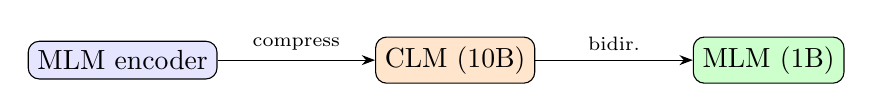
\begin{tikzpicture}[node distance=2cm, >=Stealth]
        \node[draw, rounded corners, fill=blue!10] (base) {MLM encoder};
        \node[draw, rounded corners, fill=orange!20, right=of base] (clm) {CLM (10B)};
        \node[draw, rounded corners, fill=green!20, right=of clm] (decay) {MLM (1B)};

        \draw[->] (base) -- (clm) node[midway, above] {\scriptsize compress};
        \draw[->] (clm) -- (decay) node[midway, above] {\scriptsize bidir.};
    \end{tikzpicture}
    \end{center}

    \vspace{0.3cm}
    \textbf{Why CLM first?}
    \begin{itemize}
        \item CLM: Every token predicts next $\rightarrow$ uniform gradient signal
        \item MLM: Only 15\% masked $\rightarrow$ sparse gradient signal
    \end{itemize}

    \vspace{0.2cm}
    \begin{center}
    \small
    Gradient CV: CLM = 0.12 (uniform) vs MLM = 0.59 (sparse)
    \end{center}
\end{frame}

\begin{frame}{Ch.5: CLM Improves ALL Tokens}
    \textbf{Key ablation:} Pooling strategy comparison

    \begin{table}
    \centering
    \begin{tabular}{lccc}
    \toprule
    Pooling & CLM F1 & MLM F1 & Gap \\
    \midrule
    CLS token & 23.0\% & 18.1\% & +4.9pp \\
    \textbf{Mean pooling} & \textbf{39.9\%} & 32.8\% & \textbf{+7.1pp} \\
    \bottomrule
    \end{tabular}
    \end{table}

    \vspace{0.3cm}
    \textbf{Finding:} Gap is LARGER with mean pooling (+7.1pp vs +4.9pp)

    \vspace{0.3cm}
    $\rightarrow$ CLS concentration is NOT the mechanism

    $\rightarrow$ CLM improves \textbf{all token representations}, not just CLS
\end{frame}

\begin{frame}{Ch.5: Computational Hysteresis}
    \textbf{Question:} Does MLM decay undo CLM compression?

    \begin{columns}
    \begin{column}{0.55\textwidth}
    \begin{center}
    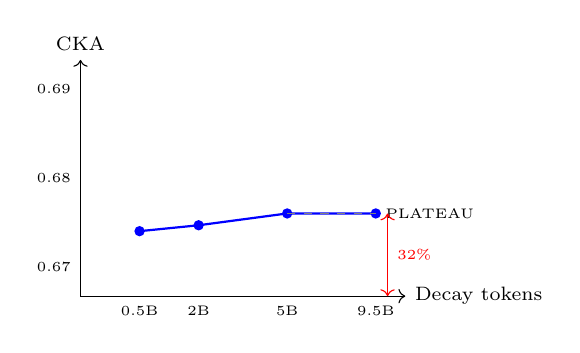
\begin{tikzpicture}[scale=0.75]
        % Axes
        \draw[->] (0,0) -- (5.5,0) node[right] {\scriptsize Decay tokens};
        \draw[->] (0,0) -- (0,4) node[above] {\scriptsize CKA};

        % Y-axis labels (CKA from 0.67 to 0.70)
        \node[left] at (0,0.5) {\tiny 0.67};
        \node[left] at (0,2) {\tiny 0.68};
        \node[left] at (0,3.5) {\tiny 0.69};

        % X-axis labels
        \node[below] at (1,0) {\tiny 0.5B};
        \node[below] at (2,0) {\tiny 2B};
        \node[below] at (3.5,0) {\tiny 5B};
        \node[below] at (5,0) {\tiny 9.5B};

        % CKA line: 0.676, 0.677, 0.679, 0.679 → scale to y: (val-0.665)*100
        % 0.676→1.1, 0.677→1.2, 0.679→1.4, 0.679→1.4
        \draw[blue, thick] (1,1.1) -- (2,1.2) -- (3.5,1.4) -- (5,1.4);
        \foreach \x/\y in {1/1.1, 2/1.2, 3.5/1.4, 5/1.4}
            \fill[blue] (\x,\y) circle (2.5pt);

        % Plateau annotation
        \draw[dashed, gray] (3.5,1.4) -- (5,1.4);
        \node[right] at (5,1.4) {\tiny PLATEAU};

        % Permanent divergence annotation
        \draw[<->, red] (5.2,0) -- (5.2,1.4);
        \node[right, red] at (5.2,0.7) {\tiny 32\%};
    \end{tikzpicture}
    \end{center}
    \end{column}

    \begin{column}{0.45\textwidth}
    \textbf{No.} CKA similarity (CLM$\rightarrow$decay vs MLM):
    \begin{itemize}
        \item 0.5B decay: 0.676
        \item 9.5B decay: 0.679
        \item $\Delta$ = +0.003 (plateau)
    \end{itemize}

    \vspace{0.3cm}
    \textbf{32\% permanent divergence}

    $\rightarrow$ CLM effects persist despite MLM decay
    \end{column}
    \end{columns}
\end{frame}

\begin{frame}{Ch.5: Non-Localizable Effect}
    \textbf{Experiment:} Transplant CLM layers into MLM model

    \begin{table}
    \centering
    \small
    \begin{tabular}{lcc}
    \toprule
    Transplant & F1 & \% of gap recovered \\
    \midrule
    + early (L0--7) & 31.9\% & $-$7\% (worse!) \\
    + mid (L8--14) & 35.3\% & \textbf{+37\%} \\
    + late (L15--21) & 32.4\% & $-$1\% (worse!) \\
    + all attention & 33.9\% & +19\% \\
    + all MLP & 35.3\% & +37\% \\
    \midrule
    \multicolumn{2}{l}{\textbf{Max recovery:}} & \textbf{37\%} \\
    \bottomrule
    \end{tabular}
    \end{table}

    \vspace{0.2cm}
    $\rightarrow$ No single component captures $>$37\% of the advantage

    $\rightarrow$ The effect is \textbf{emergent}: distributed across the entire network
\end{frame}

\begin{frame}{Ch.5: MLM Can't Exploit Rich Data}
    \textbf{Control experiment:} Same MCQA data, different objective

    \begin{table}
    \centering
    \begin{tabular}{lcc}
    \toprule
    Model & Objective & $\Delta$ vs baseline \\
    \midrule
    CLM + MCQA & CLM & \textbf{+7.1pp} \\
    MLM + MCQA & MLM & $-$2.8pp \\
    \bottomrule
    \end{tabular}
    \end{table}

    \vspace{0.3cm}
    \textbf{Finding:} MLM \textit{degrades} with instruction data

    \vspace{0.3cm}
    $\rightarrow$ MLM's sparse gradients can't exploit structured Q\&A

    $\rightarrow$ CLM's uniform coverage captures the signal
\end{frame}

\begin{frame}{Ch.5: Position Trade-off}
    \begin{columns}
    \begin{column}{0.55\textwidth}
    \begin{table}
    \centering
    \scriptsize
    \begin{tabular}{lccc}
    \toprule
    Position & CLM & MLM & $\Delta$ \\
    \midrule
    256--1024 & 0.918 & 0.873 & \textbf{+4.5\%} \\
    1024--2048 & 0.913 & 0.875 & \textbf{+3.8\%} \\
    2048--4096 & 0.723 & 0.834 & $-$11\% \\
    4096+ & 0.635 & 0.757 & $-$12\% \\
    \bottomrule
    \end{tabular}
    \end{table}
    \end{column}

    \begin{column}{0.45\textwidth}
    \begin{itemize}
        \item CLM wins at 0--2048
        \item MLM wins at 2048+
        \item Most clinical docs: 256--2048
    \end{itemize}

    \vspace{0.2cm}
    \textbf{Why?}

    Gradient imbalance in CLM:
    \begin{itemize}
        \item Early positions: over-trained
        \item Late positions: under-trained
    \end{itemize}
    \end{column}
    \end{columns}
\end{frame}

\begin{frame}{Ch.5: French Clinical Coding Results}
    \textbf{ModernCamemBERT-bio: CLM vs MLM (8 tasks, 9 seeds)}

    \begin{table}
    \centering
    \scriptsize
    \begin{tabular}{llccc}
    \toprule
    Type & Task & MCB-bio (MLM) & MCB-bio (CLM) & $\Delta$ \\
    \midrule
    ICD-10 & FRACCO-30 & 66.8 & \textbf{71.0} & +4.3pp \\
    ICD-10 & FRACCO-100 & 54.4 & \textbf{57.1} & +2.6pp \\
    SNOMED & Cantemist & 62.1 & \textbf{64.6} & +2.5pp \\
    SNOMED & Distemist & \textbf{28.1} & 23.9 & $-$4.2pp \\
    Dialog & MedDialog & 62.4 & \textbf{63.8} & +1.4pp \\
    Classif. & DiaMED & 59.3 & \textbf{64.1} & +4.8pp \\
    NER & EMEA & 69.1 & \textbf{71.2} & +2.1pp \\
    NER & Medline & 59.8 & \textbf{62.1} & +2.2pp \\
    \midrule
    \multicolumn{2}{l}{\textbf{Average}} & 57.7 & \textbf{59.7} & \textbf{+2.0pp} \\
    \bottomrule
    \end{tabular}
    \end{table}

    \vspace{0.2cm}
    CLM wins \textbf{7/8 tasks} $\rightarrow$ robust across task types
\end{frame}

\begin{frame}{Ch.5: English Results (PubMed 10B)}
    \textbf{ModernBERT-base on English biomedical benchmarks}

    \begin{table}
    \centering
    \small
    \begin{tabular}{llccc}
    \toprule
    Type & Task & MLM & CLM & $\Delta$ \\
    \midrule
    QA & PubMedQA & \textbf{47.8} & 34.6 & $-$13.2pp \\
    MCQA & MedQA & 17.6 & \textbf{18.2} & +0.6pp \\
    Classif. & GAD & 70.6 & \textbf{73.9} & +3.2pp \\
    Relation & ChemProt & 28.4 & \textbf{29.9} & +1.5pp \\
    \bottomrule
    \end{tabular}
    \end{table}

    \vspace{0.3cm}
    \textbf{CLM wins 3/4 tasks} -- similar pattern to French

    \vspace{0.3cm}
    \textbf{Exception:} QA requires bidirectional attention (question$\leftrightarrow$context)

    $\rightarrow$ CLM's causal attention hurts Q$\leftrightarrow$A reasoning
\end{frame}

% Question transition
\begin{frame}[plain]
\vfill
\begin{center}
{\large\textit{Can we also inject structured knowledge}}

\vspace{0.5cm}
{\large\textit{during pretraining?}}
\end{center}
\vfill
\end{frame}

% ========== CHAPTER 6: Knowledge-Enriched ==========
\begin{frame}{Ch.6: Ontobook Pipeline}
    \textbf{Publication:} Ontobook -- Inject ontology knowledge during pretraining

    \vspace{0.3cm}
    \begin{center}
    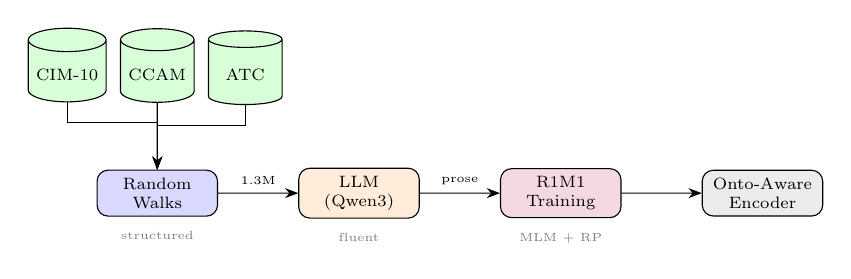
\begin{tikzpicture}[node distance=1.2cm, >=Stealth, scale=0.85, transform shape]
        % Ontologies
        \node[draw, cylinder, shape border rotate=90, aspect=0.3, fill=green!15, minimum width=1.1cm, minimum height=1.1cm, font=\scriptsize] (cim) {CIM-10};
        \node[draw, cylinder, shape border rotate=90, aspect=0.3, fill=green!15, minimum width=1.1cm, minimum height=1.1cm, right=0.2cm of cim, font=\scriptsize] (ccam) {CCAM};
        \node[draw, cylinder, shape border rotate=90, aspect=0.3, fill=green!15, minimum width=1.1cm, minimum height=1.1cm, right=0.2cm of ccam, font=\scriptsize] (atc) {ATC};

        % Walks
        \node[draw, rounded corners, fill=blue!15, below=1cm of ccam, minimum width=1.8cm, font=\scriptsize, align=center] (walks) {Random\\Walks};

        % Textbook
        \node[draw, rounded corners, fill=orange!15, right=1.2cm of walks, minimum width=1.8cm, font=\scriptsize, align=center] (textbook) {LLM\\(Qwen3)};

        % Training
        \node[draw, rounded corners, fill=purple!15, right=1.2cm of textbook, minimum width=1.8cm, font=\scriptsize, align=center] (train) {R1M1\\Training};

        % Output
        \node[draw, rounded corners, fill=gray!15, right=1.2cm of train, minimum width=1.8cm, font=\scriptsize, align=center] (output) {Onto-Aware\\Encoder};

        % Arrows
        \draw[->] (cim.south) -- ++(0,-0.3) -| (walks);
        \draw[->] (ccam.south) -- (walks);
        \draw[->] (atc.south) -- ++(0,-0.3) -| (walks);
        \draw[->] (walks) -- (textbook) node[midway, above, font=\tiny] {1.3M};
        \draw[->] (textbook) -- (train) node[midway, above, font=\tiny] {prose};
        \draw[->] (train) -- (output);

        % Labels below
        \node[below=0.1cm of walks, font=\tiny, text=gray] {structured};
        \node[below=0.1cm of textbook, font=\tiny, text=gray] {fluent};
        \node[below=0.1cm of train, font=\tiny, text=gray] {MLM + RP};
    \end{tikzpicture}
    \end{center}

    \vspace{0.2cm}
    \begin{table}
    \centering
    \scriptsize
    \begin{tabular}{lrr}
    \toprule
    Ontology & Walks & Size \\
    \midrule
    CIM-10 (diagnoses) & 402k & 2.3 GB \\
    CCAM (procedures) & 763k & 2.9 GB \\
    ATC (drugs) & 139k & 291 MB \\
    \bottomrule
    \end{tabular}
    \end{table}
\end{frame}

\begin{frame}{Ch.6: Textbook Reformulation}
    \textbf{Transform structured walk $\rightarrow$ fluent medical prose}

    \vspace{0.3cm}
    \begin{columns}
    \begin{column}{0.48\textwidth}
    \textbf{Structured Walk:}
    \begin{block}{}
    \scriptsize
    \texttt{[E11] Diabète de type 2}\\
    \texttt{>> Partie de: E10-E14}\\
    \texttt{>> À distinguer de: E10}\\
    \texttt{>> Complications: E11.2, E11.3}
    \end{block}
    \end{column}

    \begin{column}{0.04\textwidth}
    \centering
    $\Rightarrow$
    \end{column}

    \begin{column}{0.48\textwidth}
    \textbf{Fluent Textbook:}
    \begin{block}{}
    \scriptsize
    Le \textbf{diabète de type 2} (E11) appartient aux diabètes sucrés (E10-E14). Il doit être distingué du diabète de type 1 (E10). Ses complications incluent les atteintes rénales (E11.2) et ophtalmiques (E11.3).
    \end{block}
    \end{column}
    \end{columns}

    \vspace{0.4cm}
    \textbf{Training objective:}
    \begin{itemize}
        \item MLM: predict masked tokens
        \item Relation Prediction: 6 classes (parent, child, sibling, etc.)
    \end{itemize}
\end{frame}

\begin{frame}{Ch.6: Ontobook Results}
    \textbf{Finding:} +3.86 points over MLM baseline

    \begin{table}
    \centering
    \small
    \begin{tabular}{lcccc}
    \toprule
    Model & FRACCO & Cantemist & Distemist & Avg \\
    \midrule
    MLM-baseline & 55.81 & 66.01 & 24.23 & 48.68 \\
    \textbf{OntoBook} & \textbf{58.33} & \textbf{67.06} & \textbf{32.24} & \textbf{52.54} \\
    Misaligned & 33.39 & 20.11 & 12.63 & 22.04 \\
    \bottomrule
    \end{tabular}
    \end{table}

    \vspace{0.2cm}
    \textbf{Critical insights:}
    \begin{itemize}
        \item \textbf{Alignment is essential:} misaligned = $-$26.64 points (catastrophic)
        \item \textbf{Cross-ontology transfer:} ATC (drugs) improves Distemist (diseases) +8 pts
    \end{itemize}
\end{frame}

\section{Part 3: Adapting to Clinical Tasks}

\begin{frame}[plain]
\vfill
\begin{center}
{\Large\textit{How to use pretrained models with little annotation?}}
\end{center}
\vfill
\end{frame}

% ========== CHAPTER 7: Zero-Shot GLiNER ==========
\begin{frame}{Ch.7: The Problem -- Too Many Labels}
    \textbf{Clinical coding: thousands of labels}

    \begin{table}
    \centering
    \small
    \begin{tabular}{lll}
    \toprule
    Task & Ontology & Labels \\
    \midrule
    Diagnosis coding & ICD-10 & 17,000+ codes \\
    Drug coding & ATC & 6,000+ codes \\
    Procedure coding & CCAM & 8,000+ codes \\
    Entity linking & SNOMED-CT & 350,000+ concepts \\
    \bottomrule
    \end{tabular}
    \end{table}

    \vspace{0.3cm}
    \textbf{Classic BERT NER:}
    \begin{itemize}
        \item Train classifier head with N outputs (N = labels)
        \item Need annotated examples for \textit{each} label
        \item $\rightarrow$ 17k labels = impossible to annotate
    \end{itemize}
\end{frame}

\begin{frame}{Ch.7: Solution -- Bi-Encoder GLiNER}
    \textbf{Publication:} MCB-bio-embed (MCB-bio-gliner)

    \vspace{0.2cm}
    \begin{center}
    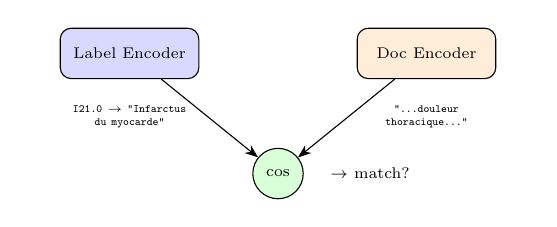
\begin{tikzpicture}[node distance=1cm, >=Stealth, scale=0.8, transform shape]
        % Label encoder
        \node[draw, rounded corners, fill=blue!15, minimum width=2.2cm, minimum height=0.8cm, font=\scriptsize, align=center] (label) {Label Encoder};
        \node[below=0.3cm of label, font=\tiny, text width=3cm, align=center] (label_ex) {\texttt{I21.0 $\rightarrow$ "Infarctus\\du myocarde"}};

        % Document encoder
        \node[draw, rounded corners, fill=orange!15, minimum width=2.2cm, minimum height=0.8cm, font=\scriptsize, align=center, right=2.5cm of label] (doc) {Doc Encoder};
        \node[below=0.3cm of doc, font=\tiny, text width=3cm, align=center] (doc_ex) {\texttt{"...douleur\\thoracique..."}};

        % Similarity
        \node[draw, circle, fill=green!15, minimum size=0.8cm, font=\scriptsize, below=1.5cm of $(label)!0.5!(doc)$] (sim) {cos};

        % Arrows
        \draw[->] (label) -- (sim);
        \draw[->] (doc) -- (sim);
        \node[right=0.3cm of sim, font=\scriptsize] {$\rightarrow$ match?};
    \end{tikzpicture}
    \end{center}

    \vspace{0.2cm}
    \textbf{Key insight:} No classifier head $\rightarrow$ zero-shot on \textit{any} label set

    \vspace{0.2cm}
    \textbf{But:} Standard GLiNER doesn't exploit ontology structure!
\end{frame}

\begin{frame}{Ch.7: WHY RDF? -- The Opportunity}
    \textbf{Problem:} Standard GLiNER ignores ontology structure

    \vspace{0.2cm}
    \textbf{RDF/SKOS gives us everything for free:}

    \begin{columns}
    \begin{column}{0.5\textwidth}
    \scriptsize
    \textbf{1. Precise code$\leftrightarrow$label:}\\
    \texttt{I21.0 $\rightarrow$ "Infarctus aigu"}

    \vspace{0.15cm}
    \textbf{2. Synonyms (positives):}\\
    \texttt{I21.0 = "IDM antérieur"}

    \vspace{0.15cm}
    \textbf{3. Hierarchy (positives):}\\
    \texttt{I21.0 $\in$ I21 (Infarctus)}
    \end{column}

    \begin{column}{0.5\textwidth}
    \scriptsize
    \textbf{4. Exclusions = hard negatives!}\\
    \texttt{I21 $\neq$ I25 "ancien infarctus"}\\
    {\tiny ``à ne pas confondre avec...''}

    \vspace{0.15cm}
    \textbf{5. Related = hard negatives!}\\
    \texttt{I21 $\neq$ I22 "récidive"}\\
    {\tiny ``exclut le code...''}
    \end{column}
    \end{columns}

    \vspace{0.3cm}
    \textbf{$\rightarrow$ Perfect for sentence transformer training:}
    \begin{itemize}
        \item 258k pairs with natural hard negatives
        \item Train specialized \textbf{label encoder} (MCB-bio-embed)
        \item Keep MCB-bio for \textbf{span prediction}
    \end{itemize}
\end{frame}

\begin{frame}{Ch.7: MCB-bio-embed Training Data}
    \textbf{Multi-source: 1.5M pairs}

    \begin{columns}
    \begin{column}{0.45\textwidth}
    \begin{table}
    \centering
    \scriptsize
    \begin{tabular}{lr}
    \toprule
    Source & Pairs \\
    \midrule
    RDF ontologies & 258k \\
    Synthetic passages & 490k \\
    Persona queries & 760k \\
    \midrule
    \textbf{Total} & \textbf{1.5M} \\
    \bottomrule
    \end{tabular}
    \end{table}
    \end{column}

    \begin{column}{0.55\textwidth}
    \scriptsize
    \textbf{Persona example:}

    \vspace{0.1cm}
    \textit{Clinicien:}\\
    ``Quelle prise en charge pour une tumeur trophoblastique?''

    \vspace{0.1cm}
    \textit{Patient:}\\
    ``C'est quoi le choriocarcinome? C'est grave?''

    \vspace{0.1cm}
    \textit{Codeur:}\\
    ``Code CIM-10 pour thrombopénie à la rifampicine?''
    \end{column}
    \end{columns}

    \vspace{0.3cm}
    $\rightarrow$ 5 personas for query diversity + hard negative mining via Solon
\end{frame}

% Question transition
\begin{frame}[plain]
\vfill
\begin{center}
{\large\textit{Good on biomedical, but worse on clinical.}}

\vspace{0.5cm}
{\large\textit{How to improve clinical performance without clinical data?}}
\end{center}
\vfill
\end{frame}

% ========== CHAPTER 8: Synthetic Clinical Data ==========
\begin{frame}{Ch.8: Synthetic Clinical Data for GLiNER}
    \textbf{Supervision:} M2 intern Anh Thu Vu (AP-HP collaboration)

    \vspace{0.2cm}
    \textbf{Problem:} Need clinical training data, but it's private

    \vspace{0.2cm}
    \textbf{Solution:} LLM generates synthetic clinical reports + annotations

    \vspace{0.3cm}
    \begin{columns}
    \begin{column}{0.5\textwidth}
    \textbf{Prompt components:}
    \begin{itemize}
        \scriptsize
        \item Admin info (age, sex, dates)
        \item ICD-10 codes (DP, DAS)
        \item Tumor info (TNM, biomarkers)
        \item NCCN treatment guidelines
        \item Note template (AP-HP style)
    \end{itemize}
    \end{column}

    \begin{column}{0.5\textwidth}
    \textbf{Generated dataset:}
    \begin{itemize}
        \scriptsize
        \item 1,000 annotated reports
        \item 46,776 entity mentions
        \item 1,554 unique entity types
        \item Median length: 1,429 tokens
    \end{itemize}
    \end{column}
    \end{columns}
\end{frame}

\begin{frame}{Ch.8: Synthetic Report Example}
    \begin{columns}
    \begin{column}{0.48\textwidth}
    \textbf{Prompt:}
    \begin{block}{}
    \tiny
    \texttt{Âge: 61, Sexe: M, Nom: L. Cornuche}\\
    \texttt{Service: CANCERO, Hôpital: Lyon Sud}\\
    \texttt{DP: Tumeur poumon (C349)}\\
    \texttt{DAS: Hémiplégie (G819)}\\
    \texttt{Stade: IV, EGFR+, ALK-, PD-L1+}\\
    \texttt{Protocole: Pemetrexed+Cisplatine}
    \end{block}
    \end{column}

    \begin{column}{0.04\textwidth}
    \centering
    $\Rightarrow$
    \end{column}

    \begin{column}{0.48\textwidth}
    \textbf{Generated note:}
    \begin{block}{}
    \tiny
    \textit{``M. Cornuche, 61 ans, HDJ pour C3 chimiothérapie. ATCD: adénocarcinome pulmonaire stade IV, métastases cérébrales, hémiplégie séquellaire. Ttt: Pemetrexed-Cisplatine. Évolution favorable, sortie domicile...''}
    \end{block}
    \end{column}
    \end{columns}

    \vspace{0.3cm}
    \textbf{Extracted entities:}\\
    {\scriptsize [MALADIE] adénocarcinome pulmonaire $\cdot$ [STADE] stade IV $\cdot$ [TRAITEMENT] Pemetrexed-Cisplatine $\cdot$ [METASTASE] métastases cérébrales}
\end{frame}

\begin{frame}{Ch.8: Physician Evaluation}
    \textbf{Blind evaluation:} 50 synthetic vs 50 real notes (10-point scale)

    \begin{table}
    \centering
    \scriptsize
    \begin{tabular}{lccccc}
    \toprule
     & Language & Coherence & Completeness & Synthesis & Overall \\
    \midrule
    \textbf{Mistral AI} & \textbf{9.33} & 7.93 & \textbf{9.67} & 8.58 & 8.40 \\
    Real (AP-HP) & 9.20 & \textbf{9.33} & 9.24 & \textbf{9.02} & \textbf{8.69} \\
    \bottomrule
    \end{tabular}
    \end{table}

    \vspace{0.2cm}
    \textbf{Key findings:}
    \begin{itemize}
        \item Synthetic data rated \textbf{more complete} than real notes (9.67 vs 9.24)
        \item Real notes have better \textbf{medical coherence} (9.33 vs 7.93)
        \item Overall quality nearly identical ($\Delta$ = 0.29)
    \end{itemize}
\end{frame}

\begin{frame}{Ch.8: GLiNER Training Results}
    \textbf{6 models trained on synthetic data}

    \begin{table}
    \centering
    \scriptsize
    \begin{tabular}{lccc}
    \toprule
    Model & Params & F1 \\
    \midrule
    GLiNER-Small & 166M & 62.05 \\
    GLiNER-Medium & 209M & 63.03 \\
    GLiNER-Multi & 209M & 63.49 \\
    \textbf{GLiNER-Large} & 459M & \textbf{64.29} \\
    GLiNER-CamemBERT-bio & 135M & 60.04 \\
    GLiNER-ModernBERT & 173M & 46.58 \\
    \bottomrule
    \end{tabular}
    \end{table}

    \vspace{0.2cm}
    \textbf{Zero-shot capability confirmed:}
    \begin{itemize}
        \item ICD codes with $<$10 occurrences: F1 = 0.61
        \item 6/44 zero-shot entity types: F1 = 1.0 (perfect)
        \item 25/44 zero-shot entities: F1 $>$ 0.5
    \end{itemize}
\end{frame}

% Question transition
\begin{frame}[plain]
\vfill
\begin{center}
{\large\textit{Can we combine ontology structure with clinical training?}}
\end{center}
\vfill
\end{frame}

% ========== CHAPTER 9: TBD ==========
\begin{frame}{Ch.9: Work in Progress}
    \textbf{Ch.9: Ontology-Aware Clinical NER}

    \vspace{0.3cm}
    \textbf{Combine insights from Ch.7 + Ch.8:}
    \begin{itemize}
        \item MCB-bio-embed label encoder (RDF-trained)
        \item Synthetic clinical data for span encoder
        \item End-to-end GLiNER with both components
    \end{itemize}

    \vspace{0.3cm}
    \textbf{Hypothesis:}
    \begin{itemize}
        \item RDF structure $\rightarrow$ better label embeddings
        \item Synthetic clinical data $\rightarrow$ better span detection
        \item Combined $\rightarrow$ best of both worlds
    \end{itemize}
\end{frame}

\begin{frame}{Contributions: Corpora \& Models}
    \textbf{Corpora:}
    \begin{itemize}
        \item biomed-fr: 413M words (French biomedical)
        \item BE-Enriched: 2M clinical paragraphs from PMC
        \item GAPeron: 3.1T tokens French web (quality-filtered)
    \end{itemize}

    \vspace{0.3cm}
    \textbf{Models:}
    \begin{itemize}
        \item CamemBERT-bio, ModernCamemBERT-bio (French encoders)
        \item BioClinical-ModernBERT (English SOTA encoder)
        \item GAPeron 1.5B / 8B / 24B (French LLMs)
        \item MCB-bio-embed (French biomedical bi-encoder)
    \end{itemize}
\end{frame}

\begin{frame}{Contributions: Methods}
    \textbf{Methods:}
    \begin{itemize}
        \item BiaHS: Benchmark-in-a-Haystack (contamination detection)
        \item CLM$\rightarrow$decay: computational hysteresis for encoder CPT
        \item OntoBook: ontology-to-textbook reformulation
        \item RDF-based sentence transformer training (MCB-bio-embed)
    \end{itemize}
\end{frame}

\begin{frame}{Contributions: Libraries}
    \textbf{TABIB} -- Tokenizer-Agnostic Biomedical Information extraction Benchmark
    \begin{itemize}
        \item Evaluate LLM vs BERT vs GLiNER fairly
        \item Evaluation NOT influenced by tokenization differences
        \item Addresses issue from CamemBERT-bio: token-level eval favors certain tokenizers
    \end{itemize}

    \vspace{0.4cm}
    \textbf{Chainette} -- Structured LLM chains with vLLM
    \begin{itemize}
        \item Pydantic typing for structured outputs
        \item Branches, nodes, routers for complex pipelines
        \item Used for: IE, reformulation, synthetic data generation
    \end{itemize}
\end{frame}

\section{Timeline}

\begin{frame}[plain]
\begin{center}
\resizebox{\textwidth}{!}{%
\begin{ganttchart}[
    hgrid,
    vgrid={*{6}{draw=none}, dotted},
    x unit=0.19cm,
    y unit chart=0.45cm,
    y unit title=0.45cm,
    title height=1,
    bar height=0.5,
    group height=0.25,
    title label font=\tiny,
    bar label font=\scriptsize,
    group label font=\scriptsize\bfseries,
    milestone label font=\scriptsize,
    time slot format=isodate,
    today=2025-02-06,
    today rule/.style={draw=red, thick, dashed},
    today label=Today,
    today label font=\tiny\itshape,
    milestone/.append style={fill=milestone, shape=diamond, inner sep=1.5pt}
]{2025-01-27}{2025-04-27}

\gantttitlecalendar{month=shortname} \\
\gantttitlecalendar{week} \\

% Thesis - Writing
\ganttgroup[group/.append style={fill=thesis!30}]{Writing}{2025-01-29}{2025-04-06} \\
\ganttbar[bar/.append style={fill=thesis}]{Related Works (3 ch.)}{2025-01-29}{2025-02-16} \\
\ganttbar[bar/.append style={fill=thesis}]{Part 1: Corpus (3 ch.)}{2025-02-17}{2025-03-02} \\
\ganttbar[bar/.append style={fill=thesis}]{Part 2: Pretraining (3 ch.)}{2025-03-03}{2025-03-16} \\
\ganttbar[bar/.append style={fill=thesis}]{Part 3: Adaptation (3 ch.)}{2025-03-17}{2025-04-06} \\

% Thesis - Final Advisor Review & Finalization
\ganttgroup[group/.append style={fill=review!30}]{Final Advisor Review}{2025-04-07}{2025-04-20} \\

\ganttbar[bar/.append style={fill=review}]{Advisor review}{2025-04-07}{2025-04-13} \\
\ganttbar[bar/.append style={fill=thesis}]{Intro + Conclusion + Abstract}{2025-04-07}{2025-04-13} \\
\ganttbar[bar/.append style={fill=review}]{Corrections}{2025-04-14}{2025-04-20} \\
\ganttmilestone{Submission}{2025-04-20}

\end{ganttchart}
}
\end{center}

\vspace{0.3cm}
\begin{center}
\scriptsize
\colorbox{thesis}{\strut\hspace{0.4em}} Writing \quad
\colorbox{review}{\strut\hspace{0.4em}} Final Advisor Review
\end{center}
\end{frame}

\begin{frame}[plain]
\begin{center}
\resizebox{\textwidth}{!}{%
\begin{ganttchart}[
    hgrid,
    vgrid={*{6}{draw=none}, dotted},
    x unit=0.19cm,
    y unit chart=0.45cm,
    y unit title=0.45cm,
    title height=1,
    bar height=0.5,
    group height=0.25,
    title label font=\tiny,
    bar label font=\scriptsize,
    group label font=\scriptsize\bfseries,
    milestone label font=\scriptsize,
    time slot format=isodate,
    today=2025-02-06,
    today rule/.style={draw=red, thick, dashed},
    today label=Today,
    today label font=\tiny\itshape,
    milestone/.append style={fill=milestone, shape=diamond, inner sep=1.5pt}
]{2025-01-27}{2025-04-27}

\gantttitlecalendar{month=shortname} \\
\gantttitlecalendar{week} \\

% Publications
\ganttgroup[group/.append style={fill=gray!20}]{Publications}{2025-01-27}{2025-04-17} \\
\ganttbar[bar/.append style={fill=done}]{Biomed-Enriched $\rightarrow$ ACL}{2025-01-27}{2025-01-27} \\
\ganttbar[bar/.append style={fill=done}]{GAPeron $\rightarrow$ ACL}{2025-01-27}{2025-01-27} \\
\ganttbar[bar/.append style={fill=todo}]{Ontobook $\rightarrow$ Clinical NLP}{2025-01-29}{2025-02-17} \\
\ganttmilestone{MCB-bio release}{2025-02-15} \\
\ganttmilestone{Clinical NLP}{2025-02-18} \\
\ganttbar[bar/.append style={fill=todo}]{ModernCamemBERT-bio $\rightarrow$ COLM}{2025-02-17}{2025-03-30} \\
\ganttmilestone{COLM}{2025-03-31} \\
\ganttbar[bar/.append style={fill=todo}]{MCB-bio-gliner $\rightarrow$ BioNLP}{2025-03-17}{2025-04-16} \\
\ganttmilestone{BioNLP}{2025-04-17}

\end{ganttchart}
}
\end{center}

\vspace{0.3cm}
\begin{center}
\scriptsize
\colorbox{done}{\strut\hspace{0.4em}} Submitted \quad
\colorbox{todo}{\strut\hspace{0.4em}} To do
\end{center}
\end{frame}

\end{document}
